% CS631 Advanced Programming in the UNIX Environment
% Author: Jan Schaumann <jschauma@netmeister.org>
% $Id: slides.tex,v 1.6 2005/09/28 02:45:29 jschauma Exp $
\special{! TeXDict begin /landplus90{true}store end }

\documentclass[xga]{xdvislides}
\usepackage[landscape]{geometry}
\usepackage{graphics}
\usepackage{graphicx}
\usepackage{colordvi}

\begin{document}
\setfontphv

%%% Headers and footers
\lhead{\slidetitle}
\chead{CS631 - Advanced Programming in the UNIX Environment}
\rhead{Slide \thepage}
\lfoot{\Gray{Lecture 05: Process Environment, Process Control}}
\cfoot{\relax}
\rfoot{\Gray{\today}}

\newcommand{\smallish}{\fontsize{16}{16}\selectfont}

\vspace*{\fill}
\begin{center}
	\Hugesize
		CS631 - Advanced Programming in the UNIX Environment\\
		-- \\
		Process Environment, Process Control \\
	\hspace*{5mm}\blueline\\ [1em]
	\Normalsize
		Department of Computer Science\\
		Stevens Institute of Technology\\
		Jan Schaumann\\
		\verb+jschauma@stevens.edu+\\
		\verb+http://www.cs.stevens.edu/~jschauma/631/+
\end{center}
\vspace*{\fill}

\subsection{Midterm!}
\vspace{1in}

\verb+https://www.cs.stevens.edu/~jschauma/cgi-bin/midterm.cgi+

\subsection{The {\tt main} function}
\vspace{.25in}
\small
\setlength{\unitlength}{1mm}
\begin{center}
	\begin{picture}(150,10)
		\thinlines
		\put(0,0){\framebox(130,10){}}
		\put(10,5){{\tt int main(int {\em argc}, char **{\em argv});}}
	\end{picture}
\end{center}
\Normalsize

\subsection{The {\tt main} function}
\vspace{.25in}
\small
\setlength{\unitlength}{1mm}
\begin{center}
	\begin{picture}(150,10)
		\thinlines
		\put(0,0){\framebox(130,10){}}
		\put(10,5){{\tt int main(int {\em argc}, char **{\em argv});}}
	\end{picture}
\end{center}
\Normalsize
\vspace{.25in}
\begin{itemize}
	\item C program started by kernel (by one of the {\tt exec} functions)
	\item special startup routine called by kernel which sets up things for {\tt main} (or whatever entrypoint is defined)
	\item {\tt argc} is a count of the number of command line arguments (including
		the command itself)
	\item {\tt argv} is an array of pointers to the arguments
	\item it is guaranteed by both ANSI C and POSIX.1 that {\tt argv[argc] == NULL}
\end{itemize}

\subsection{Process Creation}
On Linux:
\begin{verbatim}
$ cc -Wall entry.c
$ readelf -h a.out | more
ELF Header:
[...]
  Entry point address:               0x400460
  Start of program headers:          64 (bytes into file)
  Start of section headers:          4432 (bytes into file)
$ objdump -d a.out
[...]
0000000000400460 <_start>:
  400460:       31 ed                   xor    %ebp,%ebp
  400462:       49 89 d1                mov    %rdx,%r9
[...]
$
\end{verbatim}

\subsection{Process Creation}
\verb+glibc/sysdeps/x86_64/start.S+

\begin{verbatim}
0000000000401058 <_start>:
  401058:       31 ed                   xor    %ebp,%ebp
  40105a:       49 89 d1                mov    %rdx,%r9
  40105d:       5e                      pop    %rsi
  40105e:       48 89 e2                mov    %rsp,%rdx
  401061:       48 83 e4 f0             and    $0xfffffffffffffff0,%rsp
  401065:       50                      push   %rax
  401066:       54                      push   %rsp
  401067:       49 c7 c0 e0 1a 40 00    mov    $0x401ae0,%r8
  40106e:       48 c7 c1 50 1a 40 00    mov    $0x401a50,%rcx
  401075:       48 c7 c7 91 11 40 00    mov    $0x401191,%rdi
  40107c:       e8 2f 01 00 00          callq  4011b0 <__libc_start_main>
  401081:       f4                      hlt
  401082:       90                      nop
  401083:       90                      nop
\end{verbatim}

\subsection{Process Creation}
\verb+glibc/csu/lic-start.c+

\begin{verbatim}
STATIC int
LIBC_START_MAIN (int (*main) (int, char **, char ** MAIN_AUXVEC_DECL),
                 int argc, char **argv,
                 __typeof (main) init,
                 void (*fini) (void),
                 void (*rtld_fini) (void), void *stack_end)
{
[...]
  result = main (argc, argv, __environ MAIN_AUXVEC_PARAM);

  exit (result);
}
\end{verbatim}

\subsection{Process Creation}
On Linux:
\begin{verbatim}
$ cc -Wall entry.c
$ readelf -h a.out | more
ELF Header:
[...]
  Entry point address:               0x400460
  Start of program headers:          64 (bytes into file)
  Start of section headers:          4432 (bytes into file)
$ objdump -d a.out
[...]
0000000000400460 <_start>:
  400460:       31 ed                   xor    %ebp,%ebp
  400462:       49 89 d1                mov    %rdx,%r9
[...]
$
\end{verbatim}




\subsection{Process Creation}
On Linux:
\begin{verbatim}
$ cc -e foo entry.c
$ ./a.out
Foo for the win!
Memory fault
$ cc -e bar entry.c
$ ./a.out
bar rules!
$ echo $?
1
$ cc entry.c
$ ./a.out
Hooray main!
$ echo $?
13
$
\end{verbatim}

\subsection{Process Termination}
There are 8 ways for a process to terminate.
\\

Normal termination:
\begin{itemize}
	\item return from {\tt main}
	\item calling {\tt exit}
	\item calling {\tt \_exit} (or {\tt\_Exit})
	\item return of last thread from its start routine
	\item calling {\tt pthread\_exit} from last thread
\end{itemize}
\vspace{.25in}

\subsection{Process Termination}
There are 8 ways for a process to terminate.
\\

Normal termination:
\begin{itemize}
	\item return from {\tt main}
	\item calling {\tt exit}
	\item calling {\tt \_exit} (or {\tt\_Exit})
	\item return of last thread from its start routine
	\item calling {\tt pthread\_exit} from last thread
\end{itemize}
\vspace{.25in}
Abnormal termination:
\begin{itemize}
	\item calling {\tt abort}
	\item terminated by a signal
	\item response of the last thread to a cancellation request
\end{itemize}



\subsection{{\tt exit(3)} and {\tt \_exit(2)}}
\small
\setlength{\unitlength}{1mm}
\begin{center}
	\begin{picture}(150,40)
		\thinlines
		\put(0,0){\framebox(130,40){}}
		\put(10,35){{\tt \#include <stdlib.h>}}
		\put(10,29){{\tt void exit(int {\em status});}}
		\put(10,24){{\tt void \_Exit(int {\em status});}}
		\put(10,13){{\tt \#include <unistd.h>}}
		\put(10,8){{\tt void \_exit(int {\em status});}}
	\end{picture}
\end{center}
\Normalsize
\vspace{.5in}
\begin{itemize}
	\item {\tt \_exit} and {\tt \_Exit}
		\begin{itemize}
			\item return to the kernel immediately
			\item {\tt \_exit} required by POSIX.1
			\item {\tt \_Exit} required by ISO C99
			\item synonymous on Unix
		\end{itemize}
	\item {\tt exit} does some cleanup and then returns
	\item both take integer argument, aka {\em exit status}
\end{itemize}

\subsection{{\tt atexit(3)}}
\small
\setlength{\unitlength}{1mm}
\begin{center}
	\begin{picture}(150,20)
		\thinlines
		\put(0,0){\framebox(130,20){}}
		\put(10,13){{\tt \#include <stdlib.h>}}
		\put(10,5){{\tt int atexit(void (*func)({\em void}));}}
	\end{picture}
\end{center}
\Normalsize
\vspace{.5in}
\begin{itemize}
	\item Registers a function with a signature of {\tt void
		funcname(void)} to be called at exit
	\item Functions invoked in reverse order of registration
	\item Same function can be registered more than once
	\item Extremely useful for cleaning up open files,
		freeing certain resources, etc.
\end{itemize}

{\tt exit-handlers.c}

\subsection{Lifetime of a UNIX Process}
\begin{center}
	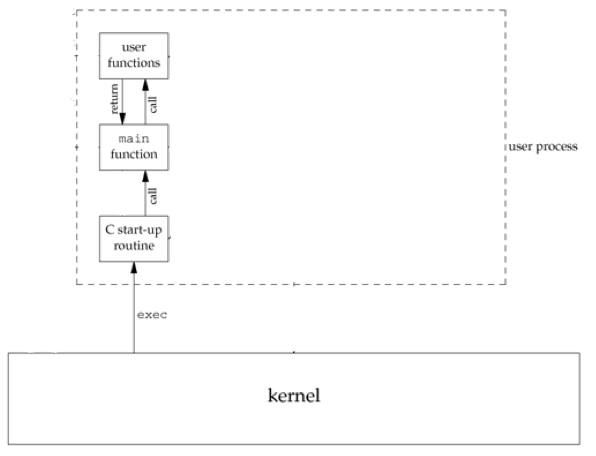
\includegraphics[angle=-90,scale=0.8]{pics/lifetime1.eps}
\end{center}

\subsection{Lifetime of a UNIX Process}
\begin{center}
	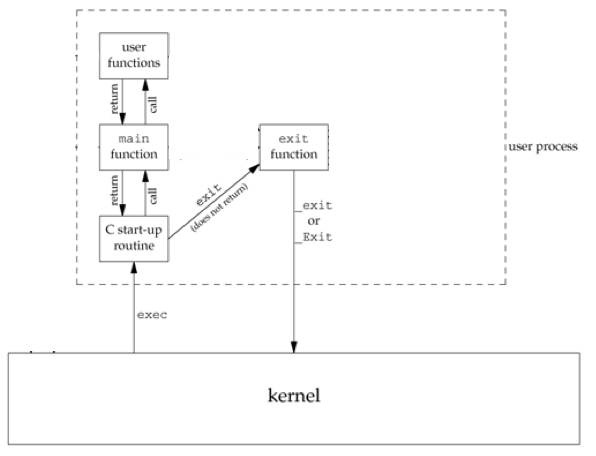
\includegraphics[angle=-90,scale=0.8]{pics/lifetime2.eps}
\end{center}

\subsection{Lifetime of a UNIX Process}
\begin{center}
	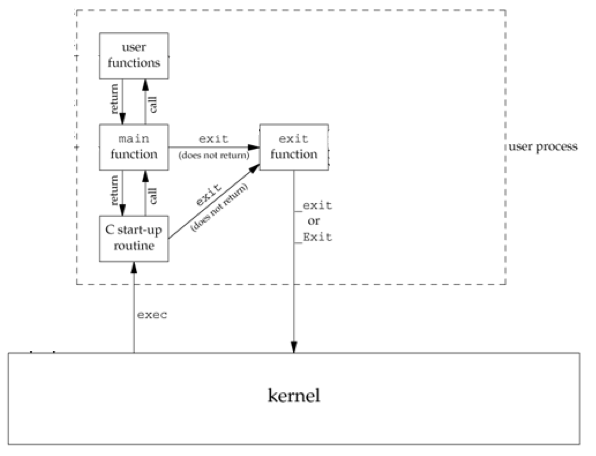
\includegraphics[angle=-90,scale=0.8]{pics/lifetime3.eps}
\end{center}

\subsection{Lifetime of a UNIX Process}
\begin{center}
	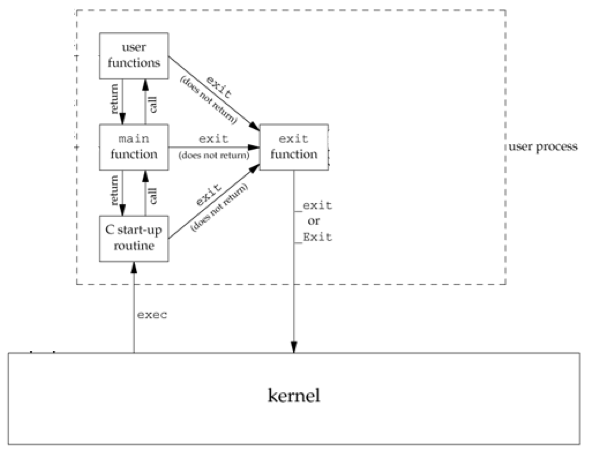
\includegraphics[angle=-90,scale=0.8]{pics/lifetime4.eps}
\end{center}

\subsection{Lifetime of a UNIX Process}
\begin{center}
	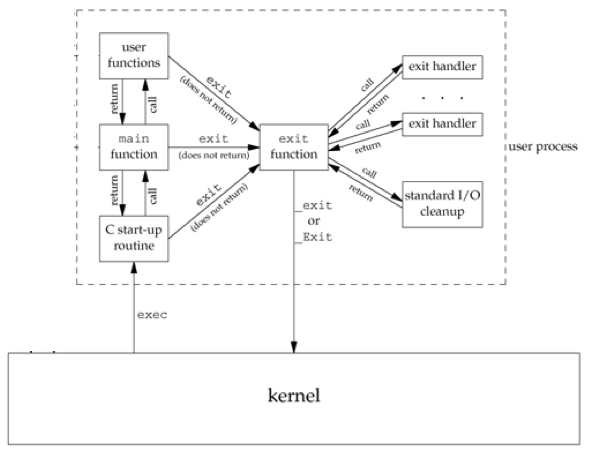
\includegraphics[angle=-90,scale=0.8]{pics/lifetime5.eps}
\end{center}

\subsection{Lifetime of a UNIX Process}
\begin{center}
	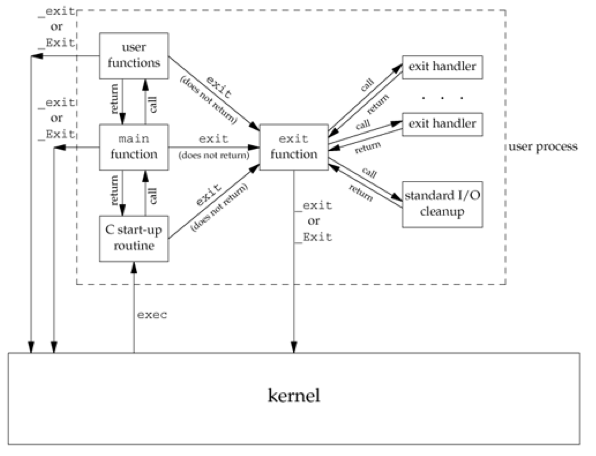
\includegraphics[angle=-90,scale=0.8]{pics/lifetime6.eps}
\end{center}

\subsection{Exit codes}
\begin{verbatim}
$ cc -Wall hw.c
hw.c: In function 'main':
hw.c:7: warning: control reaches end of non-void function
$ ./a.out
Hello World!
$ echo $?
13
$
\end{verbatim}

\subsection{Exit codes}
\begin{verbatim}
$ cc -Wall hw.c
hw.c: In function 'main':
hw.c:7: warning: control reaches end of non-void function
$ ./a.out
Hello World!
$ echo $?
10
$ cc -Wall --std=c99 hw.c
$ ./a.out
Hello World!
$ echo $?
0
$
\end{verbatim}

\subsection{Environment List}
Environment variables are stored in a global array of pointers:
\\

\verb+      extern char **environ;+
\\

The list is {\tt null} terminated.
\\

These can also be accessed by:
\vspace{.25in}
\small
\setlength{\unitlength}{1mm}
\begin{center}
	\begin{picture}(150,35)
		\thinlines
		\put(0,0){\framebox(130,35){}}
		\put(10,30){{\tt \#include <stdlib.h>}}
		\put(10,18){{\tt char *getenv(const char *{\em name});}}
		\put(10,13){{\tt int putenv(const char *{\em string});}}
		\put(10,8){{\tt int setenv(const char *{\em name}, const char *{\em value}, int {\em rewrite});}}
		\put(10,3){{\tt void unsetenv(cont char *{\em name});}}
	\end{picture}
\end{center}
\Normalsize

\subsection{Environment List}
Environment variables are stored in a global array of pointers:
\\

\verb+      extern char **environ;+
\\

The list is {\tt null} terminated.
\\

These can also be accessed by:
\vspace{.25in}
\small
\setlength{\unitlength}{1mm}
\begin{center}
	\begin{picture}(150,35)
		\thinlines
		\put(0,0){\framebox(130,35){}}
		\put(10,30){{\tt \#include <stdlib.h>}}
		\put(10,18){{\tt char *getenv(const char *{\em name});}}
		\put(10,13){{\tt int putenv(const char *{\em string});}}
		\put(10,8){{\tt int setenv(const char *{\em name}, const char *{\em value}, int {\em rewrite});}}
		\put(10,3){{\tt void unsetenv(cont char *{\em name});}}
	\end{picture}
\end{center}
\vspace{.25in}
\small
\setlength{\unitlength}{1mm}
\begin{center}
	\begin{picture}(150,10)
		\thinlines
		\put(0,0){\framebox(130,10){}}
		\put(10,5){{\tt int main(int {\em argc}, char **{\em argv}, char **{\em anvp});}}
	\end{picture}
\end{center}
\Normalsize


\Normalsize

\subsection{Memory Layout of a C Program}
\begin{center}
	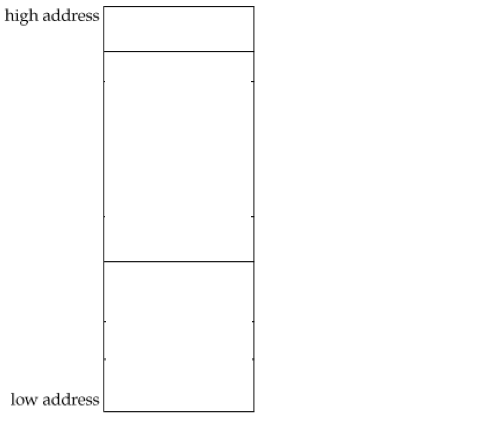
\includegraphics[angle=-90,scale=0.8]{pics/process1.eps}
\end{center}

\subsection{Memory Layout of a C Program}
\begin{center}
	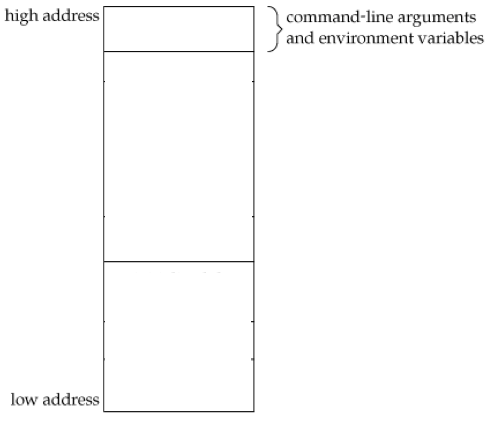
\includegraphics[angle=-90,scale=0.8]{pics/process2.eps}
\end{center}

\subsection{Memory Layout of a C Program}
\begin{center}
	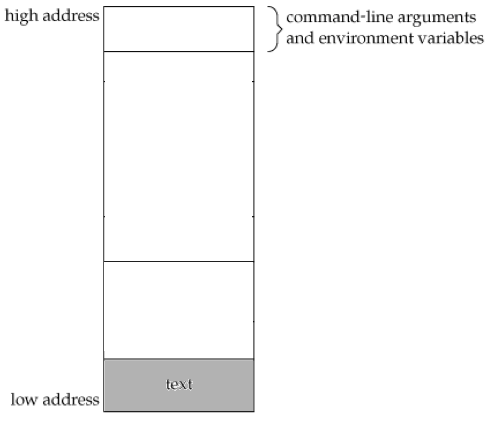
\includegraphics[angle=-90,scale=0.8]{pics/process3.eps}
\end{center}

\subsection{Memory Layout of a C Program}
\begin{center}
	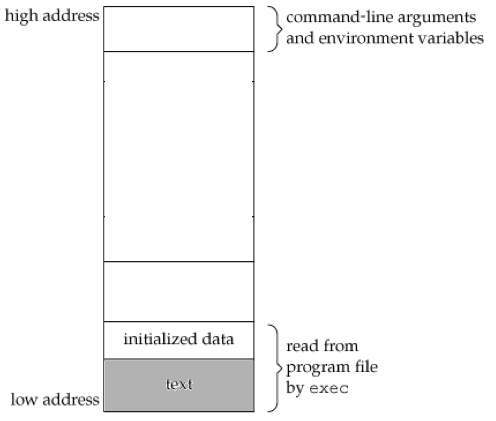
\includegraphics[angle=-90,scale=0.8]{pics/process4.eps}
\end{center}

\subsection{Memory Layout of a C Program}
\begin{center}
	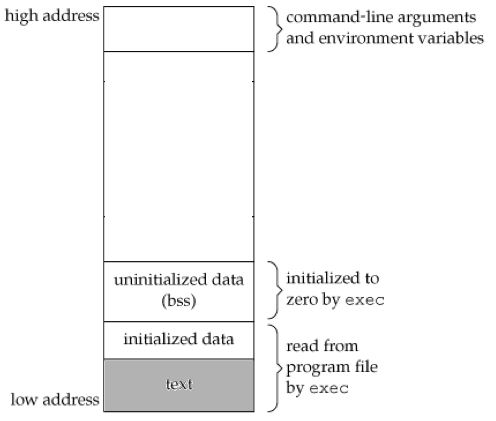
\includegraphics[angle=-90,scale=0.8]{pics/process5.eps}
\end{center}

\subsection{Memory Layout of a C Program}
\begin{center}
	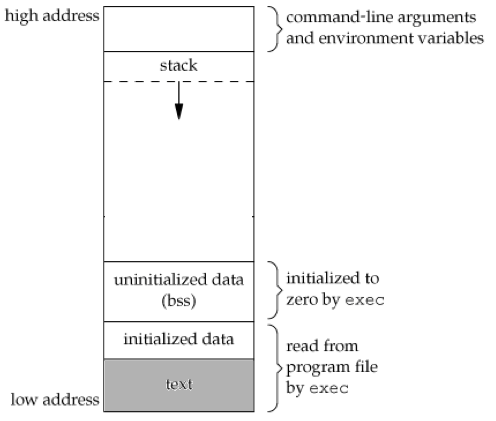
\includegraphics[angle=-90,scale=0.8]{pics/process6.eps}
\end{center}

\subsection{Memory Layout of a C Program}
\begin{center}
	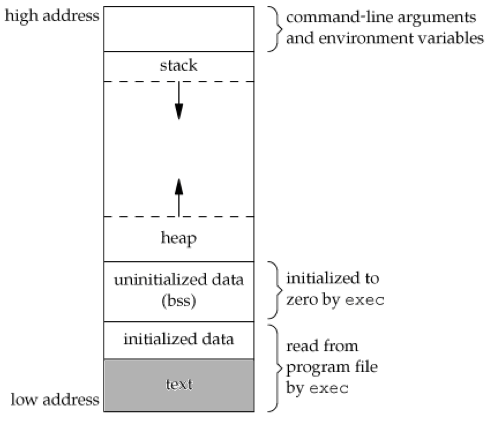
\includegraphics[angle=-90,scale=0.8]{pics/process7.eps}
\end{center}

\subsection{Memory Layout of a C Program}
\begin{center}
	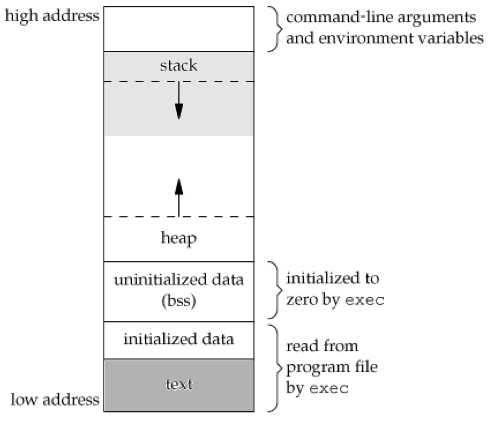
\includegraphics[angle=-90,scale=0.8]{pics/process8.eps}
\end{center}

\subsection{Memory Layout of a C Program}
\begin{center}
	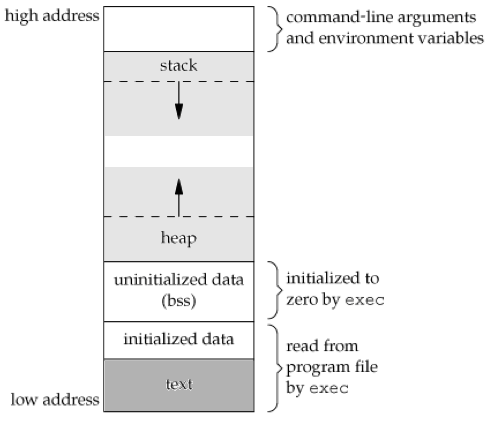
\includegraphics[angle=-90,scale=0.8]{pics/process9.eps}
\end{center}

\subsection{Memory Layout of a C Program}
On NetBSD:
\begin{verbatim}
$ cc hw.c
$ file a.out
a.out: ELF 64-bit LSB executable, x86-64, version 1 (SYSV), dynamically
linked (uses shared libs), for NetBSD 5.0, not stripped
$ ldd a.out
a.out:
        -lc.12 => /usr/lib/libc.so.12
$ size a.out
   text    data     bss     dec     hex filename
   2301     552     120    2973     b9d a.out
$ objdump -d a.out > obj
$ wc -l obj
     271 obj
$
\end{verbatim}

\subsection{Memory Layout of a C Program}
On Mac OS X:
\begin{verbatim}
$ cc hw.c
$ file a.out
a.out: Mach-O 64-bit executable x86_64
$ otool -L a.out
a.out:
	/usr/lib/libSystem.B.dylib (compatibility version 1.0.0,
current version 125.2.11)
$ size a.out
__TEXT	__DATA	__OBJC	others	dec	hex
4096	4096	0	4294971392	4294979584	100003000
$ otool -t -v a.out > obj
$ wc -l obj
      32 obj
$
\end{verbatim}

\subsection{Memory Layout of a C Program}
On Linux:
\begin{verbatim}
$ cc hw.c
$ file a.out
a.out: ELF 32-bit LSB executable, Intel 80386, version 1 (SYSV),
dynamically linked (uses shared libs), for GNU/Linux 2.6.15, not stripped
$ ldd a.out
	linux-gate.so.1 =>  (0x00c66000)
	libc.so.6 => /lib/tls/i686/cmov/libc.so.6 (0x006b4000)
	/lib/ld-linux.so.2 (0x005fe000)
$ size a.out
   text	   data	    bss	    dec	    hex	filename
    918	    264	      8	   1190	    4a6	a.out
$ objdump -d a.out >obj
$ wc -l obj
225 obj
$
\end{verbatim}

\subsection{Memory Layout of a C Program}
On NetBSD:
\begin{verbatim}
$ cc -static hw.c
$ file a.out
a.out: ELF 64-bit LSB executable, x86-64, version 1 (SYSV), statically
linked, for NetBSD 5.0, not stripped
$ ldd a.out
ldd: a.out: unrecognized file format2 [2 != 1]
$ size a.out
   text    data     bss     dec     hex filename
 151877    4416   16384  172677   2a285 a.out
$ size a.out.dyn
   text    data     bss     dec     hex filename
   2301     552     120    2973     b9d a.out
$ objdump -d a.out > obj
$ wc -l obj
   35029 obj
$
\end{verbatim}

\subsection{Memory Layout of a C Program}
On Mac OS X:
\begin{verbatim}
$ cc -static hw.c
ld: library not found for -lcrt0.o
collect2: ld returned 1 exit status
$
\end{verbatim}

\subsection{Memory Layout of a C Program}
On Linux:
\begin{verbatim}
$ cc -static hw.c
$ file a.out
a.out: ELF 32-bit LSB executable, Intel 80386, version 1 (SYSV),
statically linked, for GNU/Linux 2.6.15, not stripped
$ ldd a.out
/usr/bin/ldd: line 161: /lib64/ld-linux-x86-64.so.2: cannot execute binary file
	not a dynamic executable
$ size a.out
   text	   data	    bss	    dec	    hex	filename
 510786	   1928	   7052	 519766	  7ee56	a.out
$ objdump -d a.out >obj
$ wc -l obj
114420 obj
$
\end{verbatim}

\subsection{Memory Allocation}
\small
\setlength{\unitlength}{1mm}
\begin{center}
	\begin{picture}(150,40)
		\thinlines
		\put(0,0){\framebox(130,40){}}
		\put(10,35){{\tt \#include <stdlib.h>}}
		\put(10,28){{\tt void *malloc(size\_t {\em size});}}
		\put(10,23){{\tt void *calloc(size\_t {\em nobj}, size\_t {\em size});}}
		\put(10,18){{\tt void *realloc(void *{\em ptr}, size\_t {\em newsize});}}
		\put(10,13){{\tt void *alloca(size\_t {\em size});}}
		\put(10,5){{\tt void free(void *{\em ptr});}}
	\end{picture}
\end{center}
\Normalsize
\begin{itemize}
	\item {\em malloc} -- initial value is indeterminate.
	\item {\em calloc} -- initial value set to all zeros.
	\item {\em realloc} -- changes size of previously allocated area. Initial
		value of any additional space is indeterminate.
	\item {\em alloca} -- allocates memory on stack
\end{itemize}

\subsection{Memory Allocation}
\small
\setlength{\unitlength}{1mm}
\begin{center}
	\begin{picture}(150,40)
		\thinlines
		\put(0,0){\framebox(130,40){}}
		\put(10,35){{\tt \#include <stdlib.h>}}
		\put(10,28){{\tt void *malloc(size\_t {\em size});}}
		\put(10,23){{\tt void *calloc(size\_t {\em nobj}, size\_t {\em size});}}
		\put(10,18){{\tt void *realloc(void *{\em ptr}, size\_t {\em newsize});}}
		\put(10,13){{\tt void *alloca(size\_t {\em size});}}
		\put(10,5){{\tt void free(void *{\em ptr});}}
	\end{picture}
\end{center}
\Normalsize
\begin{itemize}
	\item {\em malloc} -- initial value is indeterminate.
	\item {\em calloc} -- initial value set to all zeros.
	\item {\em realloc} -- changes size of previously allocated area. Initial
		value of any additional space is indeterminate.
	\item {\em alloca} -- allocates memory on stack
\end{itemize}
\addvspace{.5in}
Knowing this, how does manipulation of the environment work?

%\subsection{Lifetime of a UNIX Process}
%\begin{center}
%	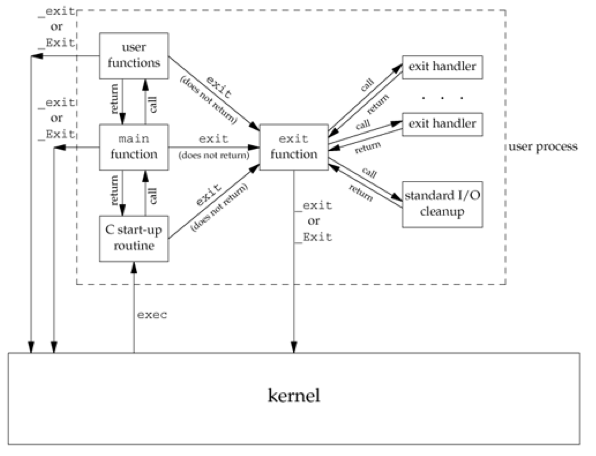
\includegraphics[angle=-90,scale=0.8]{pics/lifetime6.eps}
%\end{center}
%

% This section can be included if the students appear to have sufficient
% background knowledge so that this class does not become too advanced;
% alternatively, thSection {\tt setjmp/longjmp} taken from is might be
% added in the next lecture on signals.
%
% \verb+http://www.cs.utk.edu/~plank/plank/classes/cs360/360/notes/Setjmp/lecture.html+
%
%\subsection{{\tt setjmp(3)} and {\tt longjmp(3)}}
%\small
%\setlength{\unitlength}{1mm}
%\begin{center}
%	\begin{picture}(150,20)
%		\thinlines
%		\put(0,0){\framebox(130,20){}}
%		\put(10,15){{\tt \#include <setjmp.h>}}
%		\put(10,7){{\tt int setjmp(jmp\_buf {\em env});}}
%		\put(10,2){{\tt int longjmp(jmp\_buf {\em env}, inv {\em val});}}
%	\end{picture}
%\end{center}
%\Normalsize
%
%Things you {\em can} (but not necessarily {\em should}) do using these
%functions:
%\begin{itemize}
%	\item use as ``non-local goto''
%	\item handle error conditions in deeply nested functions
%		(poor man's / fake exceptions)
%	\item jump out of a signal handler back into your program
%	\item fake multi-threading
%\end{itemize}
%
%{\bf Remember}: {\tt longjmp} may not be called after the routine which
%called {\tt setjmp}.
%
%\subsection{{\tt setjmp(3)} and {\tt longjmp(3)}}
%\small
%\setlength{\unitlength}{1mm}
%\begin{center}
%	\begin{picture}(150,20)
%		\thinlines
%		\put(0,0){\framebox(130,20){}}
%		\put(10,15){{\tt \#include <setjmp.h>}}
%		\put(10,7){{\tt int setjmp(jmp\_buf {\em env});}}
%		\put(10,2){{\tt int longjmp(jmp\_buf {\em env}, inv {\em val});}}
%	\end{picture}
%\end{center}
%\Normalsize
%
%Things you {\em can} (but not necessarily {\em should}) do using these
%functions:
%\begin{itemize}
%	\item use as ``non-local goto''
%	\item handle error conditions in deeply nested functions
%		(poor man's / fake exceptions)
%	\item jump out of a signal handler back into your program
%	\item fake multi-threading
%\end{itemize}
%
%{\bf Remember}: {\tt longjmp} may not be called after the routine which
%called {\tt setjmp}.
%
%\begin{verbatim}
%setjmp() and sigsetjmp() make programs hard to understand and
%maintain.  If possible an alternative should be used.
%\end{verbatim}
%
%
%\subsection{{\tt setjmp(3)} and {\tt longjmp(3)}}
%\begin{verbatim}
%$ cc -Wall setjmp1.c
%$ ./a.out
%i = 0
%i = 2
%$
%\end{verbatim}
%
%\subsection{{\tt setjmp(3)} and {\tt longjmp(3)}}
%\begin{verbatim}
%$ cc -Wall setjmp2.c
%$ ./a.out 1 2 3 4
%proc_1(1, 2, 3, 4) = 4
%$ ./a.out 0 0 0 0
%Error -- bad value of i (0), j (0), k (0), l (0)
%$
%\end{verbatim}
%
%\subsection{{\tt setjmp(3)} and {\tt longjmp(3)}}
%\begin{verbatim}
%$ cc -Wall setjmp3.c
%$ ./a.out
%Setjmp returned -- i = 0
%In hex: 80486a6
%Jim
%s = Jim
%In B: i=3.  Calling longjmp(env, i)
%Setjmp returned -- i = 3
%In hex: 3
%Memory fault
%$
%\end{verbatim}

\subsection{Process limits}
\begin{verbatim}
$ ulimit -a
time(cpu-seconds)    unlimited
file(blocks)         unlimited
coredump(blocks)     unlimited
data(kbytes)         262144
stack(kbytes)        2048
lockedmem(kbytes)    249913
memory(kbytes)       749740
nofiles(descriptors) 128
processes            160
vmemory(kbytes)      unlimited
sbsize(bytes)        unlimited
$
\end{verbatim}

\subsection{{\tt getrlimit(2)} and {\tt setrlimit(2)}}
\small
\setlength{\unitlength}{1mm}
\begin{center}
	\begin{picture}(150,25)
		\thinlines
		\put(0,0){\framebox(130,25){}}
		\put(10,20){{\tt \#include <sys/resource.h>}}
		\put(10,12){{\tt int getrlimit(int {\em resouce}, struct rlimit *{\em rlp});}}
		\put(10,8){{\tt int setrlimit(int {\em resouce}, const struct rlimit *{\em rlp});}}
	\end{picture}
\end{center}
\Normalsize
Changing resource limits follows these rules:
\begin{itemize}
	\item a {\em soft limit} can be changed by any process to a value less
		than or equal to its hard limit
	\item any process can lower its {\em hard limit} greater than or equal to
		its soft limit
	\item only superuser can raise {\em hard limits}
	\item changes are per process only
\end{itemize}

\subsection{{\tt getrlimit(2)} and {\tt setrlimit(2)}}
\small
\setlength{\unitlength}{1mm}
\begin{center}
	\begin{picture}(150,25)
		\thinlines
		\put(0,0){\framebox(130,25){}}
		\put(10,20){{\tt \#include <sys/resource.h>}}
		\put(10,12){{\tt int getrlimit(int {\em resouce}, struct rlimit *{\em rlp});}}
		\put(10,8){{\tt int setrlimit(int {\em resouce}, const struct rlimit *{\em rlp});}}
	\end{picture}
\end{center}
\Normalsize
Changing resource limits follows these rules:
\begin{itemize}
	\item a {\em soft limit} can be changed by any process to a value less
		than or equal to its hard limit
	\item any process can lower its {\em hard limit} greater than or equal to
		its soft limit
	\item only superuser can raise {\em hard limits}
	\item changes are per process only (which is why {\tt ulimit} is a
		shell built-in)
\end{itemize}



\subsection{Process Control}
Review from our first class, the world's simplest shell:
\small
\begin{verbatim}
int
main(int argc, char **argv)
{
    char buf[1024];
    pid_t pid;
    int status;

    while (getinput(buf, sizeof(buf))) {
        buf[strlen(buf) - 1] = '\0';

        if((pid=fork()) == -1) {
            fprintf(stderr, "shell: can't fork: %s\n",
                        strerror(errno));
            continue;
        } else if (pid == 0) {
            /* child */
            execlp(buf, buf, (char *)0);
            fprintf(stderr, "shell: couldn't exec %s: %s\n", buf,
                        strerror(errno));
            exit(EX_DATAERR);
        }

        if ((pid=waitpid(pid, &status, 0)) < 0)
            fprintf(stderr, "shell: waitpid error: %s\n",
                strerror(errno));
    }

    exit(EX_OK);
}
\end{verbatim}
\Normalsize

\subsection{Process Identifiers}
\small
\setlength{\unitlength}{1mm}
\begin{center}
	\begin{picture}(150,20)
		\thinlines
		\put(0,0){\framebox(130,20){}}
		\put(10,15){{\tt \#include <unistd.h>}}
		\put(10,8){{\tt pid\_t getpid(void);}}
		\put(10,3){{\tt pid\_t getppid(void);}}
	\end{picture}
\end{center}
\Normalsize
\vspace{.25in}
{\em Process ID}'s are guaranteed to be unique and identify a particular executing
process with a non-negative integer.
\vspace{.25in}

Certain processes have fixed, special identifiers. They are:
\begin{itemize}
	\item {\em swapper}, process ID 0 -- responsible for scheduling
    \item {\em init}, process ID 1 -- bootstraps a Unix system, owns orphaned processes
    \item {\em pagedaemon}, process ID 2 -- responsible for the VM system (some Unix systems)
\end{itemize}

\subsection{{\tt fork(2)}}
\small
\setlength{\unitlength}{1mm}
\begin{center}
	\begin{picture}(150,15)
		\thinlines
		\put(0,0){\framebox(130,15){}}
		\put(10,10){{\tt \#include <unistd.h>}}
		\put(10,3){{\tt pid\_t fork(void);}}
	\end{picture}
\end{center}
\Normalsize

{\tt fork(2)} causes creation of a new process.  The new process (child
process) is an exact copy of the calling process (parent process) except for
the following:

\begin{itemize}
	\item The child process has a unique process ID.
	\item The child process has a different parent process ID (i.e., the
		process ID of the parent process).
	\item The child process has its own copy of the parent's descriptors.
	\item The child process' resource utilizations are set to 0.
\end{itemize}

{\bf Note}: no order of execution between child and parent is guaranteed!

\subsection{{\tt fork(2)}}
\begin{center}
	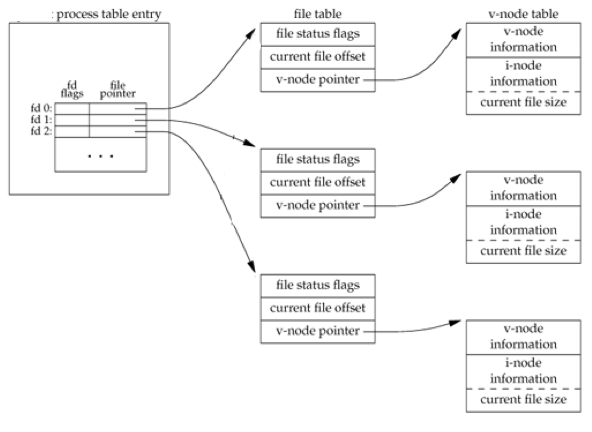
\includegraphics[angle=-90,scale=0.8]{pics/fork1.eps}
\end{center}

\subsection{{\tt fork(2)}}
\begin{center}
	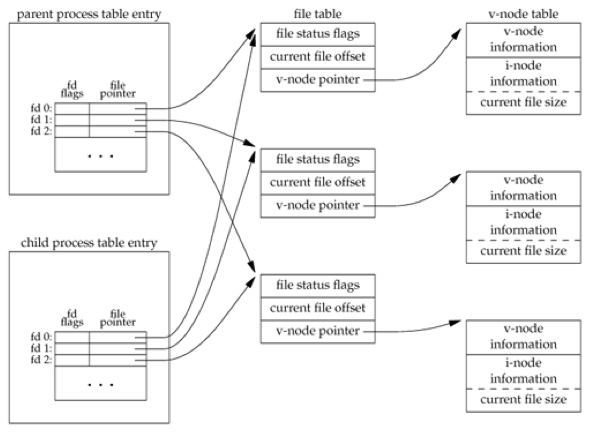
\includegraphics[angle=-90,scale=0.8]{pics/fork2.eps}
\end{center}

\subsection{{\tt fork(2)}}
\begin{verbatim}
$ cc -Wall forkflush.c
$ ./a.out
a write to stdout
before fork
pid = 12149, glob = 7, var = 89
pid = 12148, glob = 6, var = 88
$ ./a.out | cat
a write to stdout
before fork
pid = 12153, glob = 7, var = 89
before fork
pid = 12151, glob = 6, var = 88
$
\end{verbatim}

\subsection{The {\tt exec(3)} functions}
\small
\setlength{\unitlength}{1mm}
\begin{center}
	\begin{picture}(220,50)
		\thinlines
		\put(0,0){\framebox(200,50){}}
		\put(10,45){{\tt \#include <unistd.h>}}
		\put(10,38){{\tt int execl(const char *{\em pathname}, const char *{\em arg0}, ... /* (char *) 0 */);}}
		\put(10,31){{\tt int execv(const char *{\em pathname}, char * const {\em argvp[]});}}
		\put(10,24){{\tt int execle(const char *{\em pathname}, const char *{\em arg0}, ... /* (char *) 0, char
*const {\em envp[]} */ );}}
		\put(10,17){{\tt int execve(const char *{\em pathname}, char * const {\em argvp[]}, char * const {\em envp[]});}}
		\put(10,10){{\tt int execlp(const char *{\em filename}, const char *{\em arg0}, ... /* (char *) 0 */);}}
		\put(10,3){{\tt int execvp(const char *{\em filename}, char *const {\em argv[]});}}
	\end{picture}
\end{center}
\Normalsize

The {\tt exec()} family of functions are used to completely replace a running
process with a a new executable.
\begin{itemize}
	\item if it has a v in its name, argv's are a vector: {\tt const * char argv[]}
	\item if it has an l in its name, argv's are a list: {\tt const char *arg0, ... /* (char *) 0 */}
	\item if it has an e in its name, it takes a {\tt char * const envp[]} array of environment variables
	\item if it has a p in its name, it uses the {\tt PATH} environment variable to search for the file
\end{itemize}

%\subsection{{\tt vfork(2)} and {\tt COW}}
%
%While Unix has no notion of an atomic {\tt spawn} operation, the sequence:
%{\tt fork()}, {\tt exec()} is still extremely common.  A special purpose {\tt
%fork()}, called {\tt vfork()} was added in early versions of Unix.  {\tt
%vfork()}'s purpose was to create an additional process which promised to
%immediately call {\tt exec()}. Because of this promise, {\tt vfork()} was able
%to get away with not copying the heap, data, stack, bss, etc.  of the parent.
%\\
%%
%However, in the modern, more mature VM model, this ``copying'' is never done
%until an explicit write to a segment is made. Even then, only the page
%(usually around 4096 or 8192 bytes) which contains the data is copied. This
%strategy is known as ``Copy On Write'' or ``{\bf COW}''. This model
%essentially obseletes {\tt vfork()}.

\subsection{{\tt wait(2)} and {\tt waitpid(2)}}
\small
\setlength{\unitlength}{1mm}
\begin{center}
	\begin{picture}(150,40)
		\thinlines
		\put(0,0){\framebox(150,40){}}
		\put(10,35){{\tt \#include <sys/types.h>}}
		\put(10,30){{\tt \#include <sys/wait.h>}}
		\put(10,23){{\tt pid\_t wait(int *{\em status});}}
		\put(10,18){{\tt pid\_t waitpid(pid\_t {\em wpid}, int *{\em status}, int {\em options});}}
		\put(10,13){{\tt pid\_t wait3(int *{\em status}, int {\em options}, struct rusage *{\em rusage});}}
		\put(10,8){{\tt pid\_t wait4(pid\_t {\em wpid}, int *{\em status}, int {\em options}, struct rusage *{\em rusage});}}
	\end{picture}
\end{center}
\Normalsize

A parent that calls {\tt wait(2)} or {\tt waitpid(2)} can:

\begin{itemize}
	\item block (if all of its children are still running)
	\item return immediately with the termination status of a child
	\item return immediately with an error
\end{itemize}

\subsection{{\tt wait(2)} and {\tt waitpid(2)}}
Differences between {\tt wait(2)}, {\tt wait3(2)}, {\tt wait4(2)} and {\tt
waitpid(2)}:

\begin{itemize}
	\item {\tt wait(2)} will block until the process terminates, {\tt waitpid(2)}
		has an option to prevent it from blocking
	\item {\tt waitpid(2)} can wait for a specific process to finish
	\item {\tt wait3(2)} and {\tt wait4(2)} allow you to get detailed
		resource utilization statistics
	\item {\tt wait3(2)} is the same as {\tt wait4(2)} with a {\em wpid}
		value of {\tt -1}
\end{itemize}

\subsection{{\tt wait(2)} and {\tt waitpid(2)}}
Once we get a termination status back in {\tt status}, we'd like to be able to
determined how a child died. We do this with the following macros:

\begin{itemize}
	\item {\tt WIFEXITED(status)} -- true if the child terminated normally.
		Then execute {\tt WEXITSTATUS(status)} to get the exit status.
	\item {\tt WIFSIGNALED(status)} -- true if child terminated abnormally
		(by receiving a signal it didn't catch). The we call:
		\begin{itemize}
			\item {\tt WTERMSIG(status)} to retrieve the signal number
			\item {\tt WCOREDUMP(status)} to see if the child left a core image
		\end{itemize}
	\item {\tt WIFSTOPPED(status)} -- true if the child is currently stopped.
		Call {\tt WSTOPSIG(status)} to determine the signal that caused this.
\end{itemize}

Additionally, {\tt waitpid}'s behavior can be modified by supplying {\tt
WNOHANG} as an option, which says that if the requested pid has not
terminated, return immediately instead of blocking.

\subsection{What if we don't {\tt wait(2)}?}

\subsection{What if we don't {\tt wait(2)}?}
\vspace*{\fill}
\begin{center}
	
\includegraphics[scale=1.8]{pics/zombies.eps}
\end{center}
\vspace*{\fill}

\subsection{What if we don't {\tt wait(2)}?}
\smallish
\begin{verbatim}
$ cc -Wall zombies.c
$ ./a.out
Let's create some zombies!
====
15603 s003  S+     0:00.00 ./a.out
15604 s003  Z+     0:00.00 (a.out)
====
15603 s003  S+     0:00.00 ./a.out
15604 s003  Z+     0:00.00 (a.out)
15608 s003  Z+     0:00.00 (a.out)
====
15603 s003  S+     0:00.00 ./a.out
15604 s003  Z+     0:00.00 (a.out)
15612 s003  Z+     0:00.00 (a.out)
====
15603 s003  S+     0:00.00 ./a.out
15604 s003  Z+     0:00.00 (a.out)
15612 s003  Z+     0:00.00 (a.out)
15616 s003  Z+     0:00.00 (a.out)

\end{verbatim}

\subsection{Notes and Homework}

Reading:
\begin{itemize}
	\item Stevens, Chapter 7 and 8
\end{itemize}
Other:
\begin{itemize}
	\item work on your midterm project!
\end{itemize}


\end{document}
